\subsection{Thread}
\subsubsection{Protection}
\textbf{Simple Protection: Base and Bound (B\&B)}
\begin{figure}[H]
    \centering
    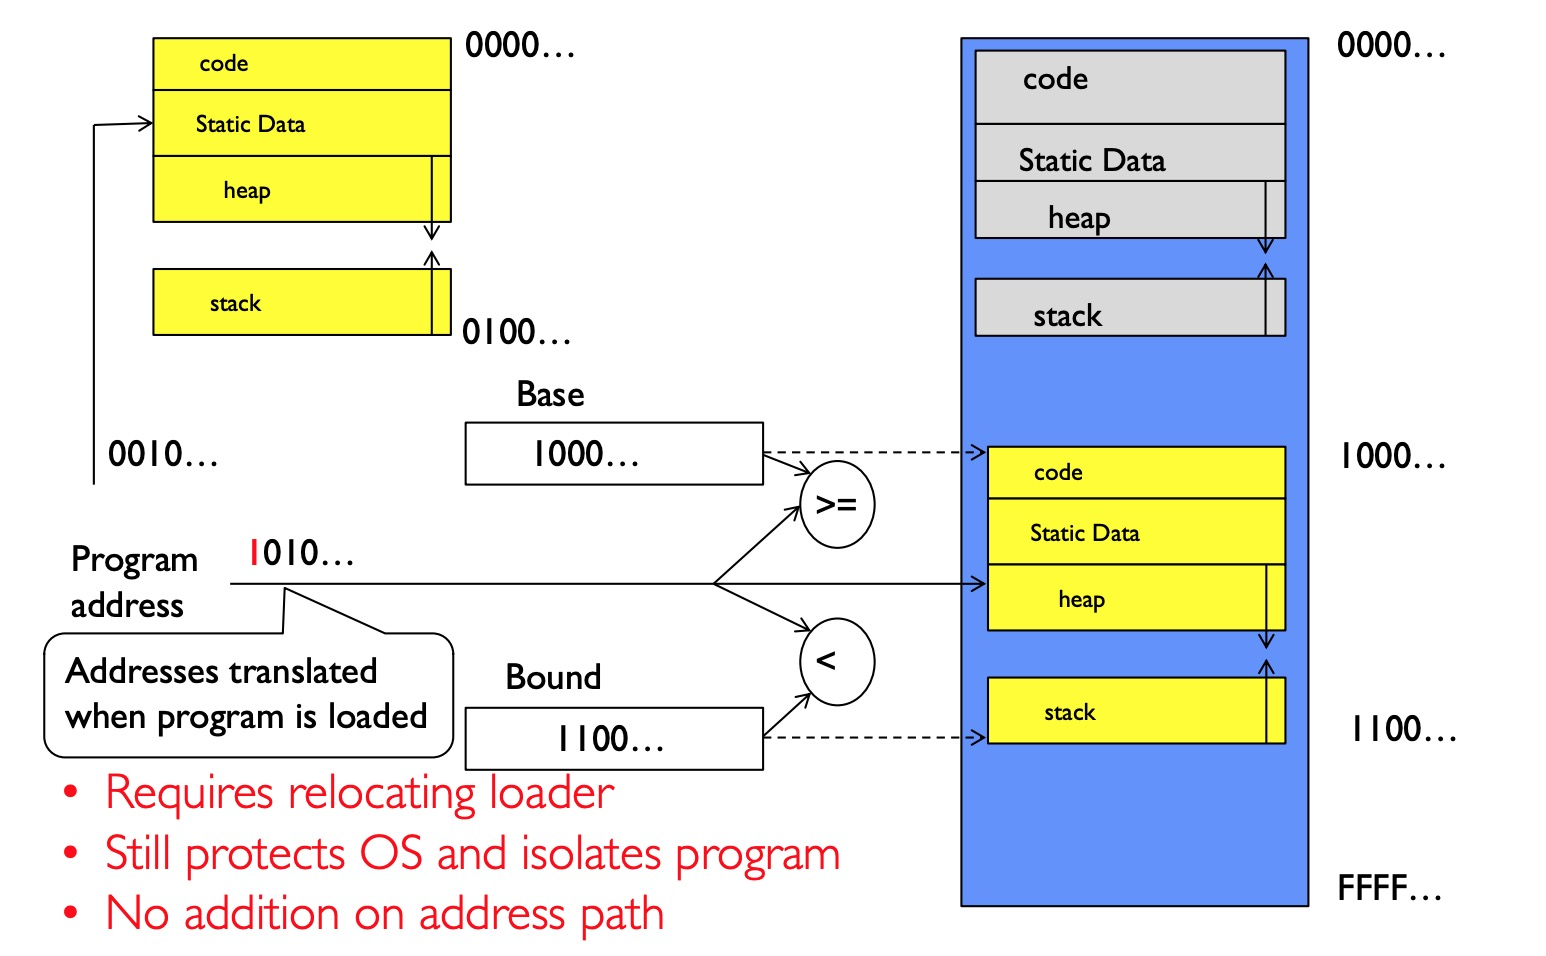
\includegraphics[width = 0.6\textwidth ]{figures/base_bound.jpg}
    \caption{Base and Bound}
    % \label{fig:batteryIncreas}
\end{figure}

\textbf{Another idea: Address Space Translation}
Program operates in an address space that is \textbf{distinct from the physical memory space of the machine}
\begin{figure}[H]
    \centering
    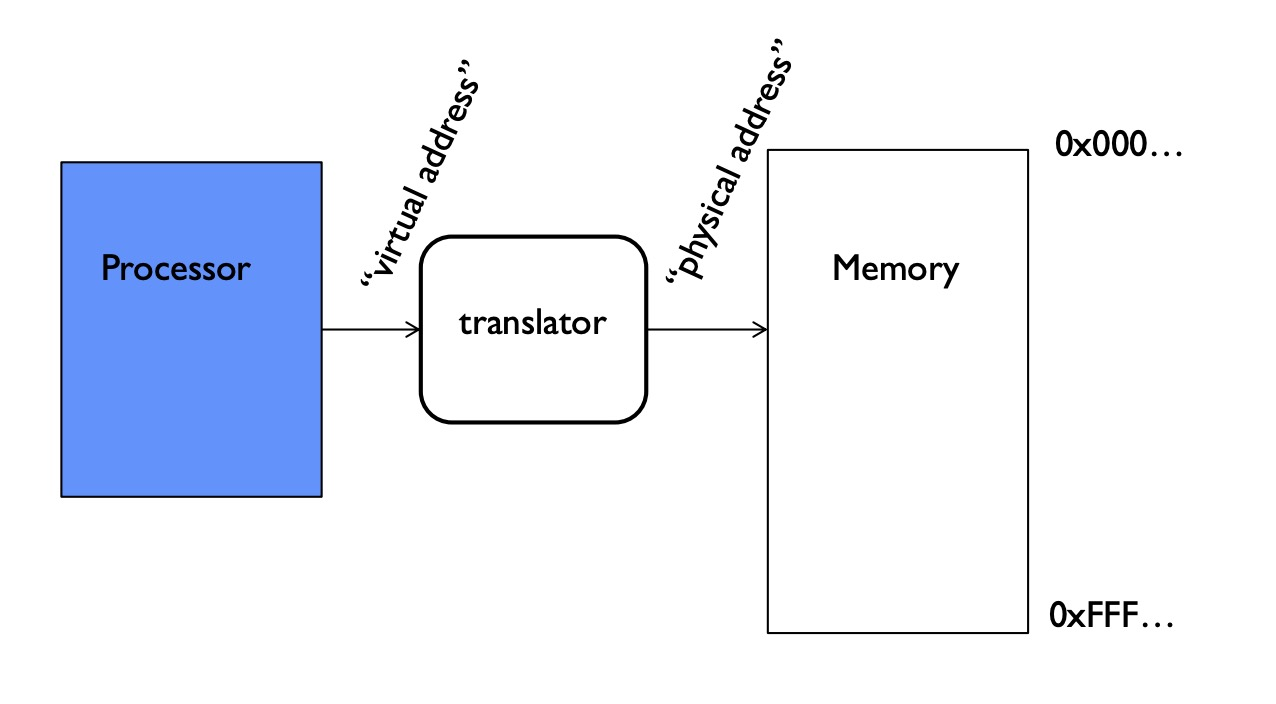
\includegraphics[width = 0.6\textwidth ]{figures/address_space_translation.jpg}
    \caption{Address Space Translation}
    % \label{fig:batteryIncreas}
\end{figure}

\begin{tcolorbox}
\begin{discussion}
How do we get the system target address of the
``unprogrammed control transfer?''
\end{discussion}    
\textbf{Interrupt Vector}
\end{tcolorbox}
\begin{example}
How does the context switch?
\end{example}

\begin{figure}[http]
\centering
\begin{minipage}[t]{0.48\textwidth}
    \centering
    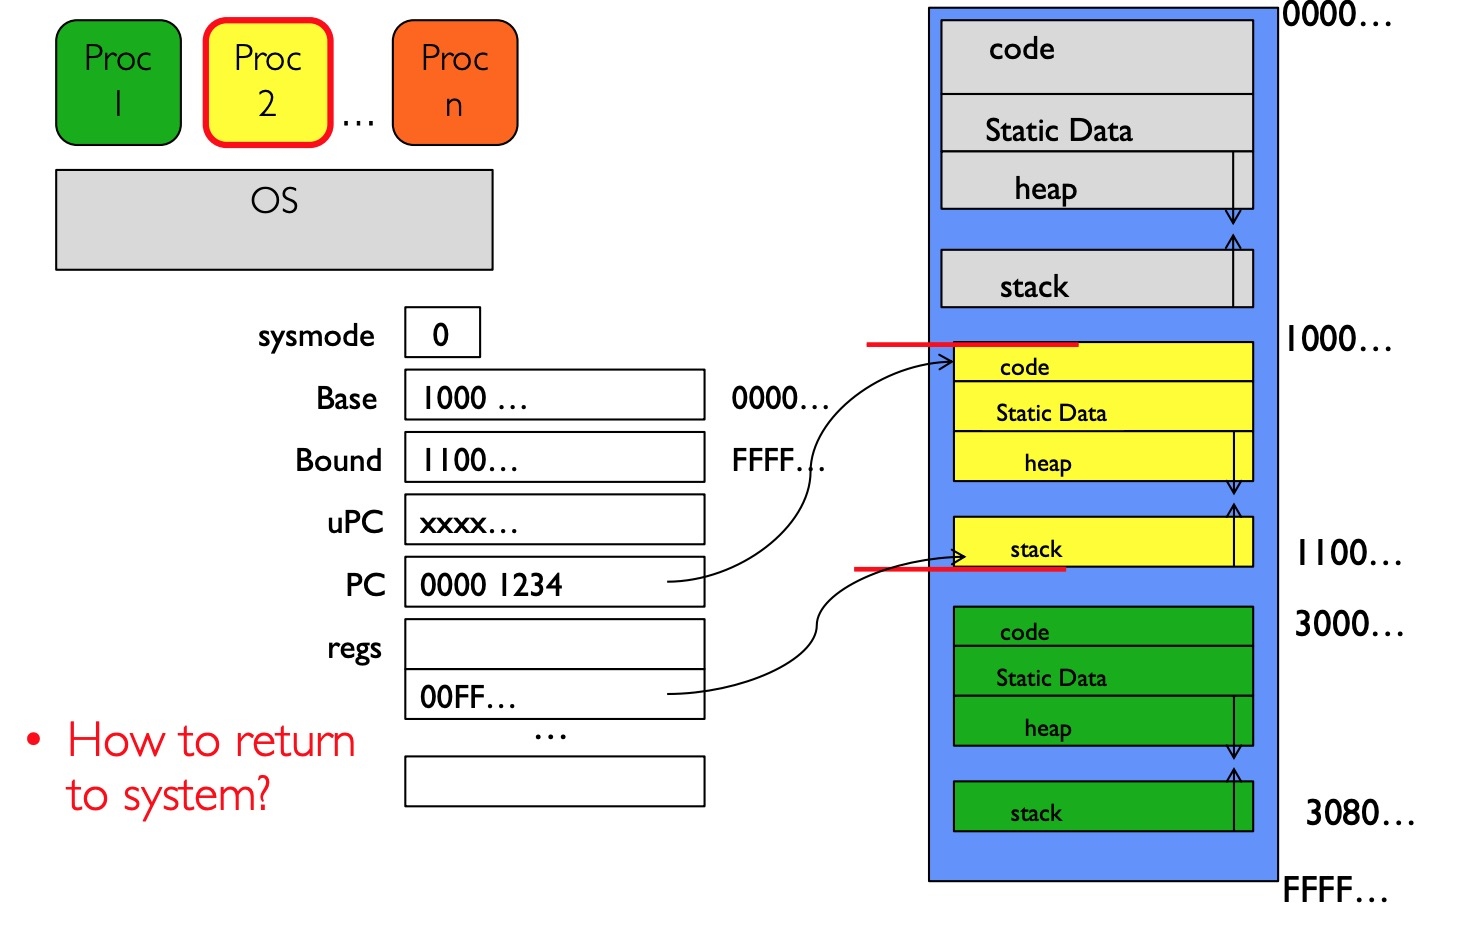
\includegraphics[width=7cm]{figures/from_user_to_kernel.jpg}
    \caption{From User to Kernel}
    % \label{fig:batteryIncreas}
    \end{minipage}
\begin{minipage}[t]{0.48\textwidth}
    \centering
    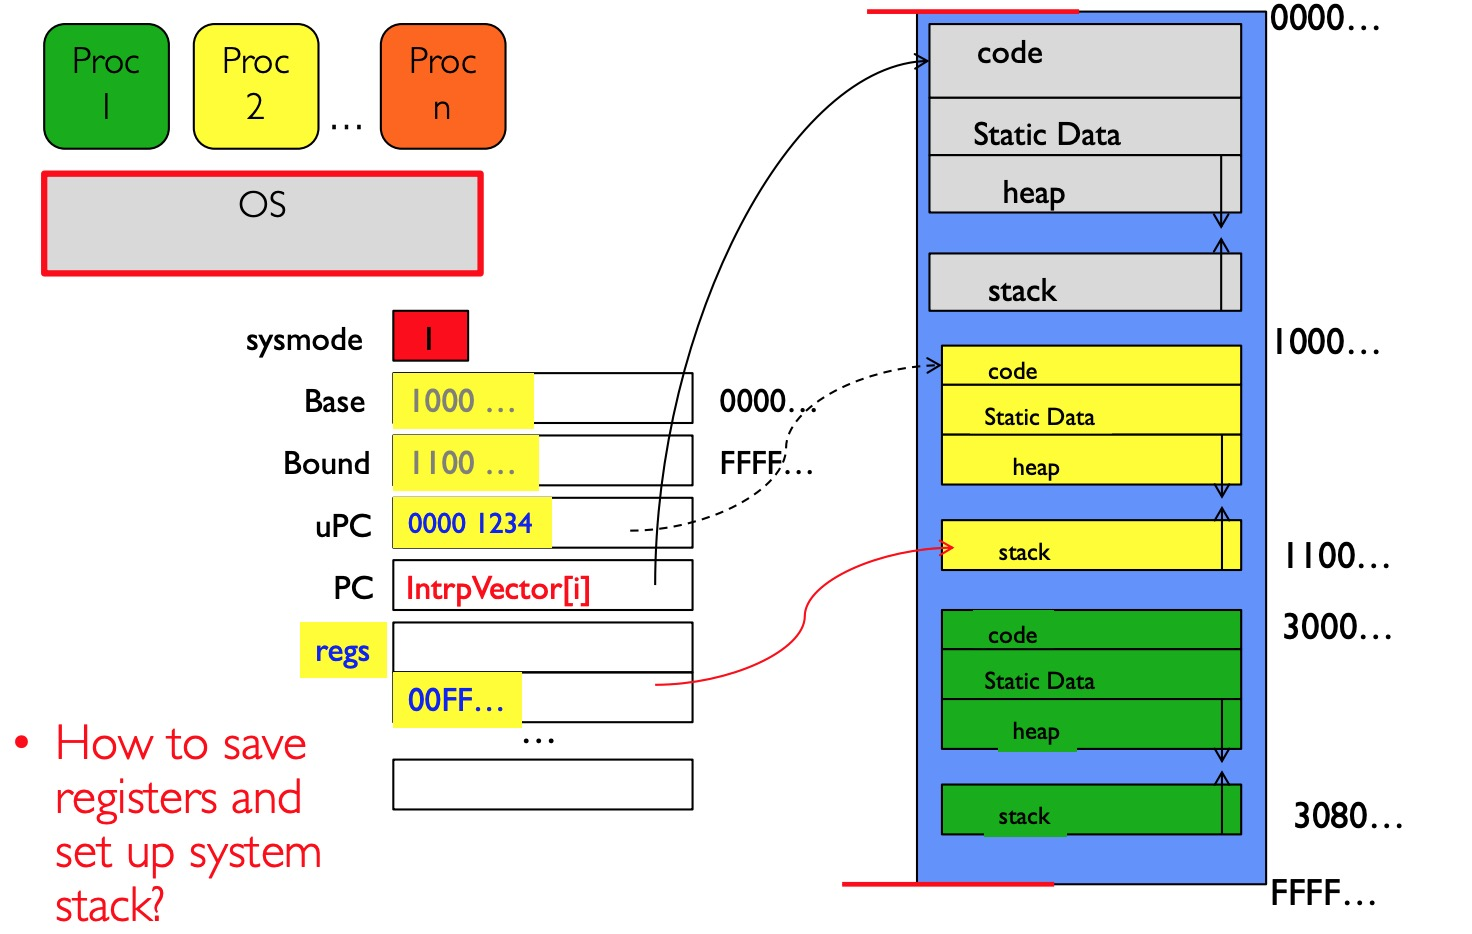
\includegraphics[width=7cm]{figures/interupt.jpg}
    \caption{Interrupt}
    % \label{fig:batteryIncreas}
    \end{minipage}
\end{figure}

\begin{figure}[http]
\centering
\begin{minipage}[t]{0.48\textwidth}
    \centering
    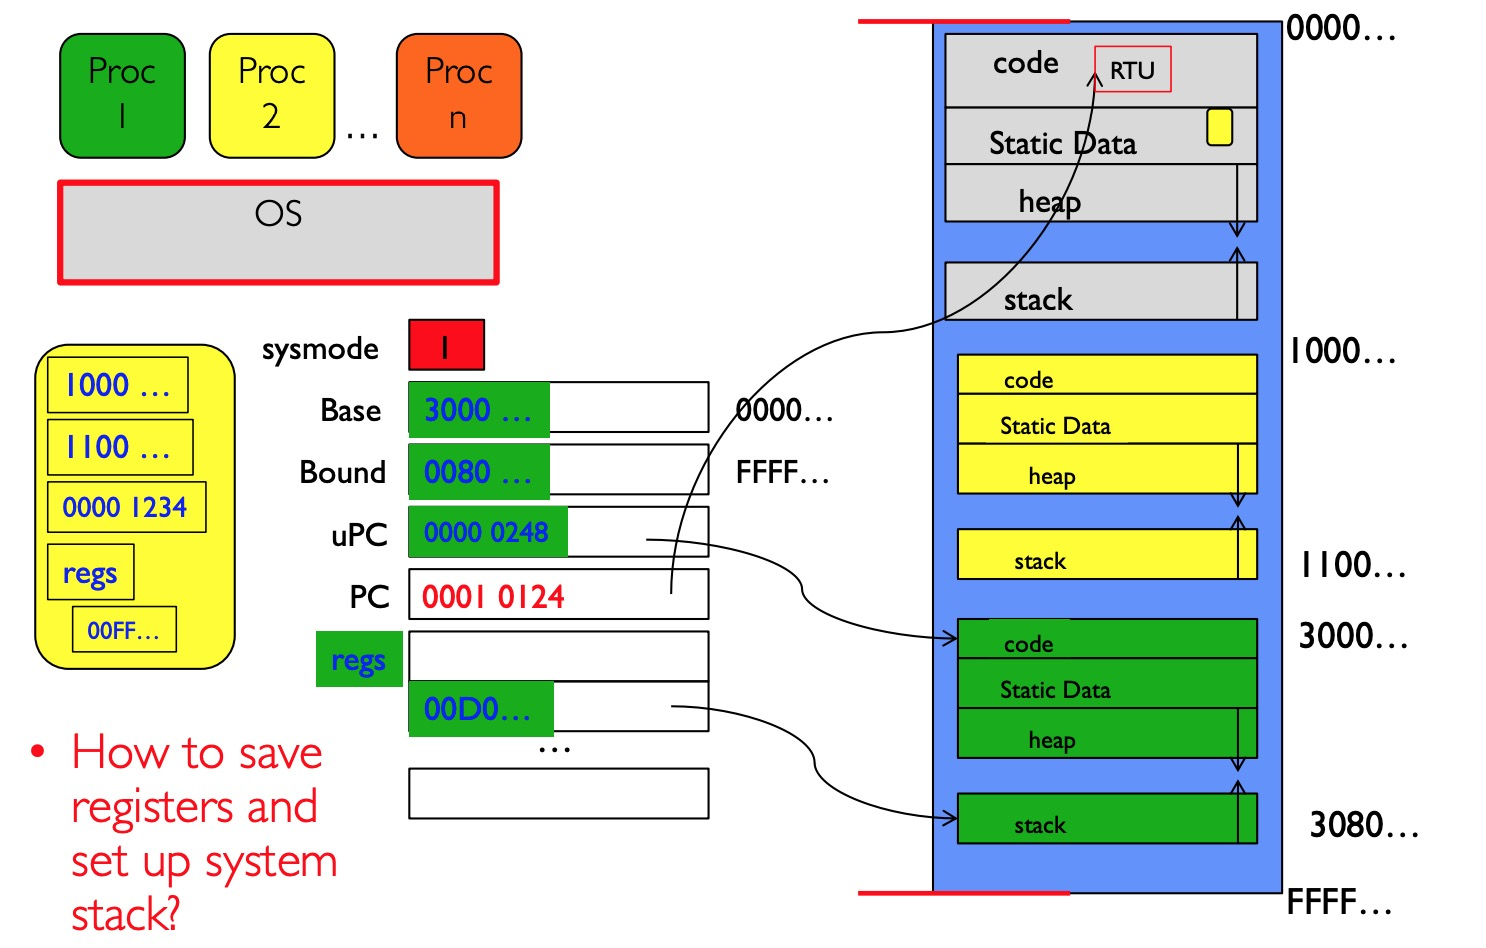
\includegraphics[width=7cm]{figures/switch.jpg}
    \caption{Switch User Process}
    % \label{fig:batteryIncreas}
    \end{minipage}
\begin{minipage}[t]{0.48\textwidth}
    \centering
    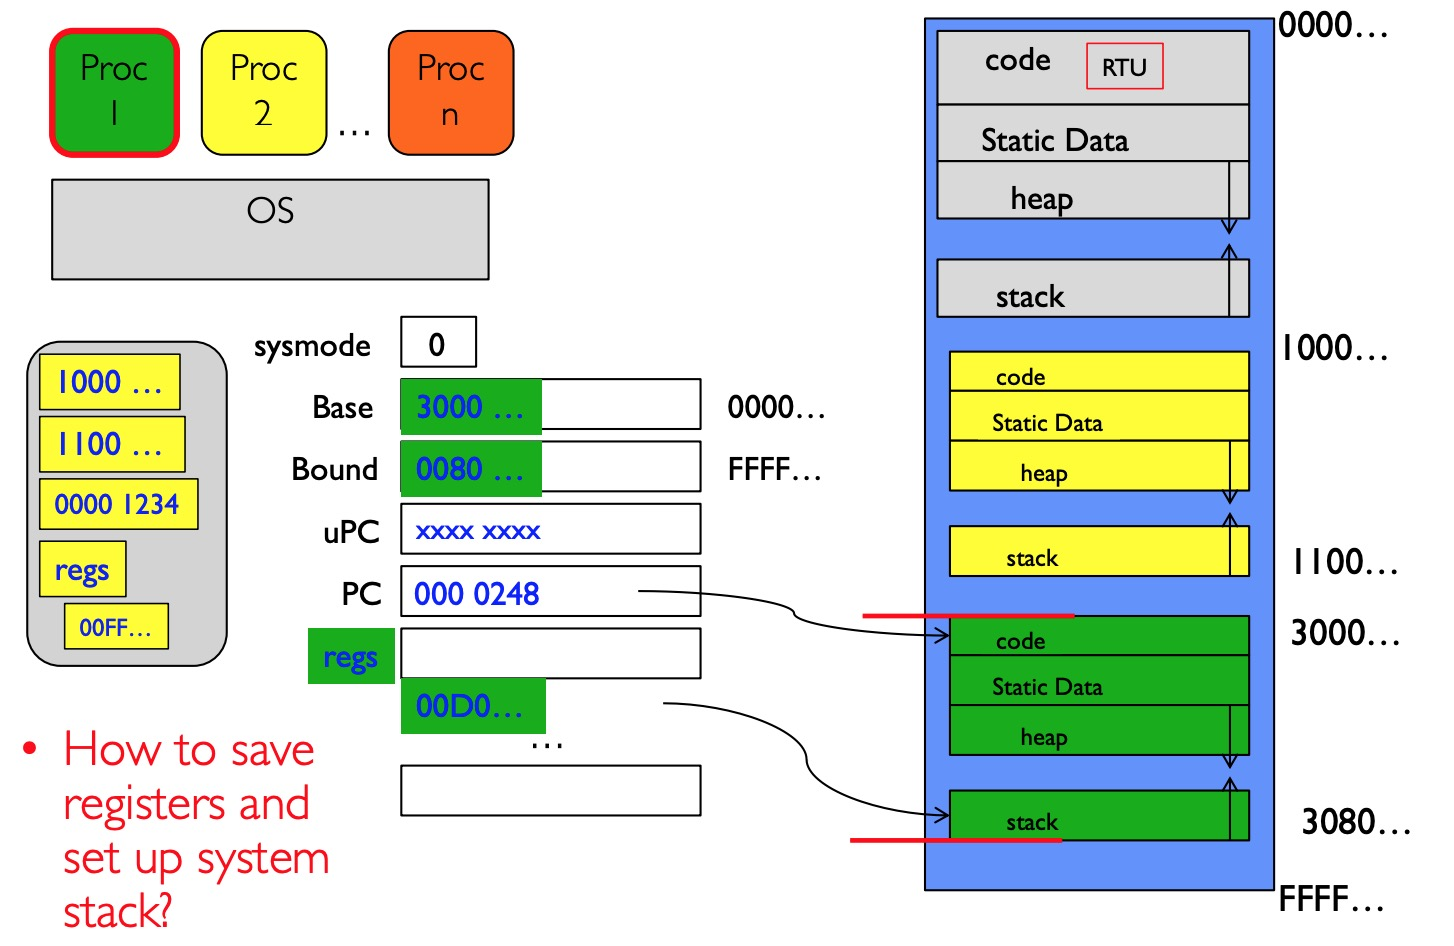
\includegraphics[width=7cm]{figures/resume.jpg}
    \caption{Resume}
    % \label{fig:batteryIncreas}
    \end{minipage}
\end{figure}
\subsubsection{Motivation for Threads}
Operating systems must handle multiple things at once (\textbf{MTAO})
\begin{itemize}
    \item Processes, interrupts, background system maintenance
\end{itemize}
Networked servers must handle \textbf{MTAO}
\begin{itemize}
    \item Multiple connections handled simultaneously
\end{itemize}
Parallel programs must handle \textbf{MTAO}
\begin{itemize}
    \item To achieve better performance
\end{itemize}
Programs with user interface often must handle \textbf{MTAO}
\begin{itemize}
    \item To achieve user responsiveness while doing computation
\end{itemize}
Network and disk bound programs must handle \textbf{MTAO}
\begin{itemize}
    \item To hide network/disk latency
    \item Sequence steps in access or communication
\end{itemize}

\begin{tcolorbox}
\begin{discussion}
Multiprocessing vs. Multiprogramming
\end{discussion}
\begin{itemize}
    \item \textbf{Multiprocessing}: Multiple CPUs (cores)
    \item \textbf{Multiprogramming}: Multiple jobs/processes
    \item \textbf{Multithreading}: Multiple threads/processes
\end{itemize}
\end{tcolorbox}

\subsubsection{Thread State}
State shared by all threads in process/address space
\begin{itemize}
    \item Content of memory (global variables, heap)
    \item I/O state (file descriptors, network connections, etc)
\end{itemize}

State “private” to each thread
\begin{itemize}
    \item Kept in \textbf{TCB} (Thread Control Block)
    \item CPU \textbf{registers} (including, program counter)
    \item Execution \textbf{stack}
\end{itemize}
